\documentclass[tikz,border=4mm]{standalone}
\usetikzlibrary{arrows.meta,positioning}
\begin{document}
\pagecolor{white}
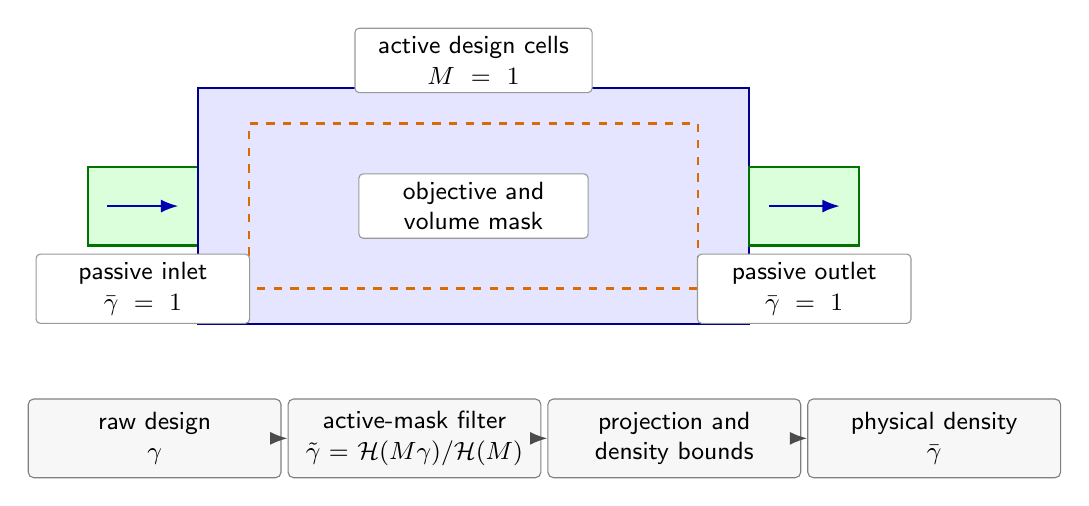
\begin{tikzpicture}[
	font=\sffamily\small,
	active/.style={draw=blue!55!black, fill=blue!10, line width=0.8pt},
	passive/.style={draw=green!45!black, fill=green!14, line width=0.8pt},
	mask/.style={draw=orange!85!black, dashed, line width=0.95pt},
	labelbox/.style={draw=black!40, fill=white, rounded corners=1.5pt, inner sep=3pt, align=center},
	processbox/.style={draw=black!50, fill=gray!6, rounded corners=2pt, minimum height=10mm, text width=30mm, align=center, inner sep=3pt},
	arrow/.style={-{Latex[length=2.2mm]}, line width=0.65pt, draw=black!70}
]

% Fixed computational domain with active and passive density regions.
\fill[passive] (-1.4,1.0) rectangle (0,2.0);
\fill[active] (0,0) rectangle (7.0,3.0);
\fill[passive] (7.0,1.0) rectangle (8.4,2.0);

\foreach \x in {0.5,1.0,...,6.5} {
	\draw[blue!24, line width=0.25pt] (\x,0) -- (\x,3);
}
\foreach \y in {0.5,1.0,...,2.5} {
	\draw[blue!24, line width=0.25pt] (0,\y) -- (7,\y);
}

\draw[passive] (-1.4,1.0) rectangle (0,2.0);
\draw[active] (0,0) rectangle (7.0,3.0);
\draw[passive] (7.0,1.0) rectangle (8.4,2.0);
\draw[mask] (0.65,0.45) rectangle (6.35,2.55);

\draw[arrow, blue!70!black] (-1.15,1.5) -- (-0.25,1.5);
\draw[arrow, blue!70!black] (7.25,1.5) -- (8.15,1.5);

\node[labelbox, text width=28mm] at (3.5,3.35) {active design cells\\$M=1$};
\node[labelbox, text width=25mm] at (-0.7,0.45) {passive inlet\\$\bar{\gamma}=1$};
\node[labelbox, text width=25mm] at (7.7,0.45) {passive outlet\\$\bar{\gamma}=1$};
\node[labelbox, text width=27mm] at (3.5,1.5) {objective and\\volume mask};

% Density map used around passive regions.
\node[processbox] (raw) at (-0.55,-1.45) {raw design\\$\gamma$};
\node[processbox] (filter) at (2.75,-1.45) {active-mask filter\\$\tilde{\gamma}=\mathcal{H}(M\gamma)/\mathcal{H}(M)$};
\node[processbox] (bounds) at (6.05,-1.45) {projection and\\density bounds};
\node[processbox] (physical) at (9.35,-1.45) {physical density\\$\bar{\gamma}$};

\draw[arrow] (raw) -- (filter);
\draw[arrow] (filter) -- (bounds);
\draw[arrow] (bounds) -- (physical);

\end{tikzpicture}
\end{document}
